\section{Arquitectura de la red distribuida}
El siguiente diagrama muestra la arquitectura prevista del sistema:
\begin{figure}[!htbp]
	\hypertarget{fig:cap1}{\hspace{1pt}}
	\begin{center}
		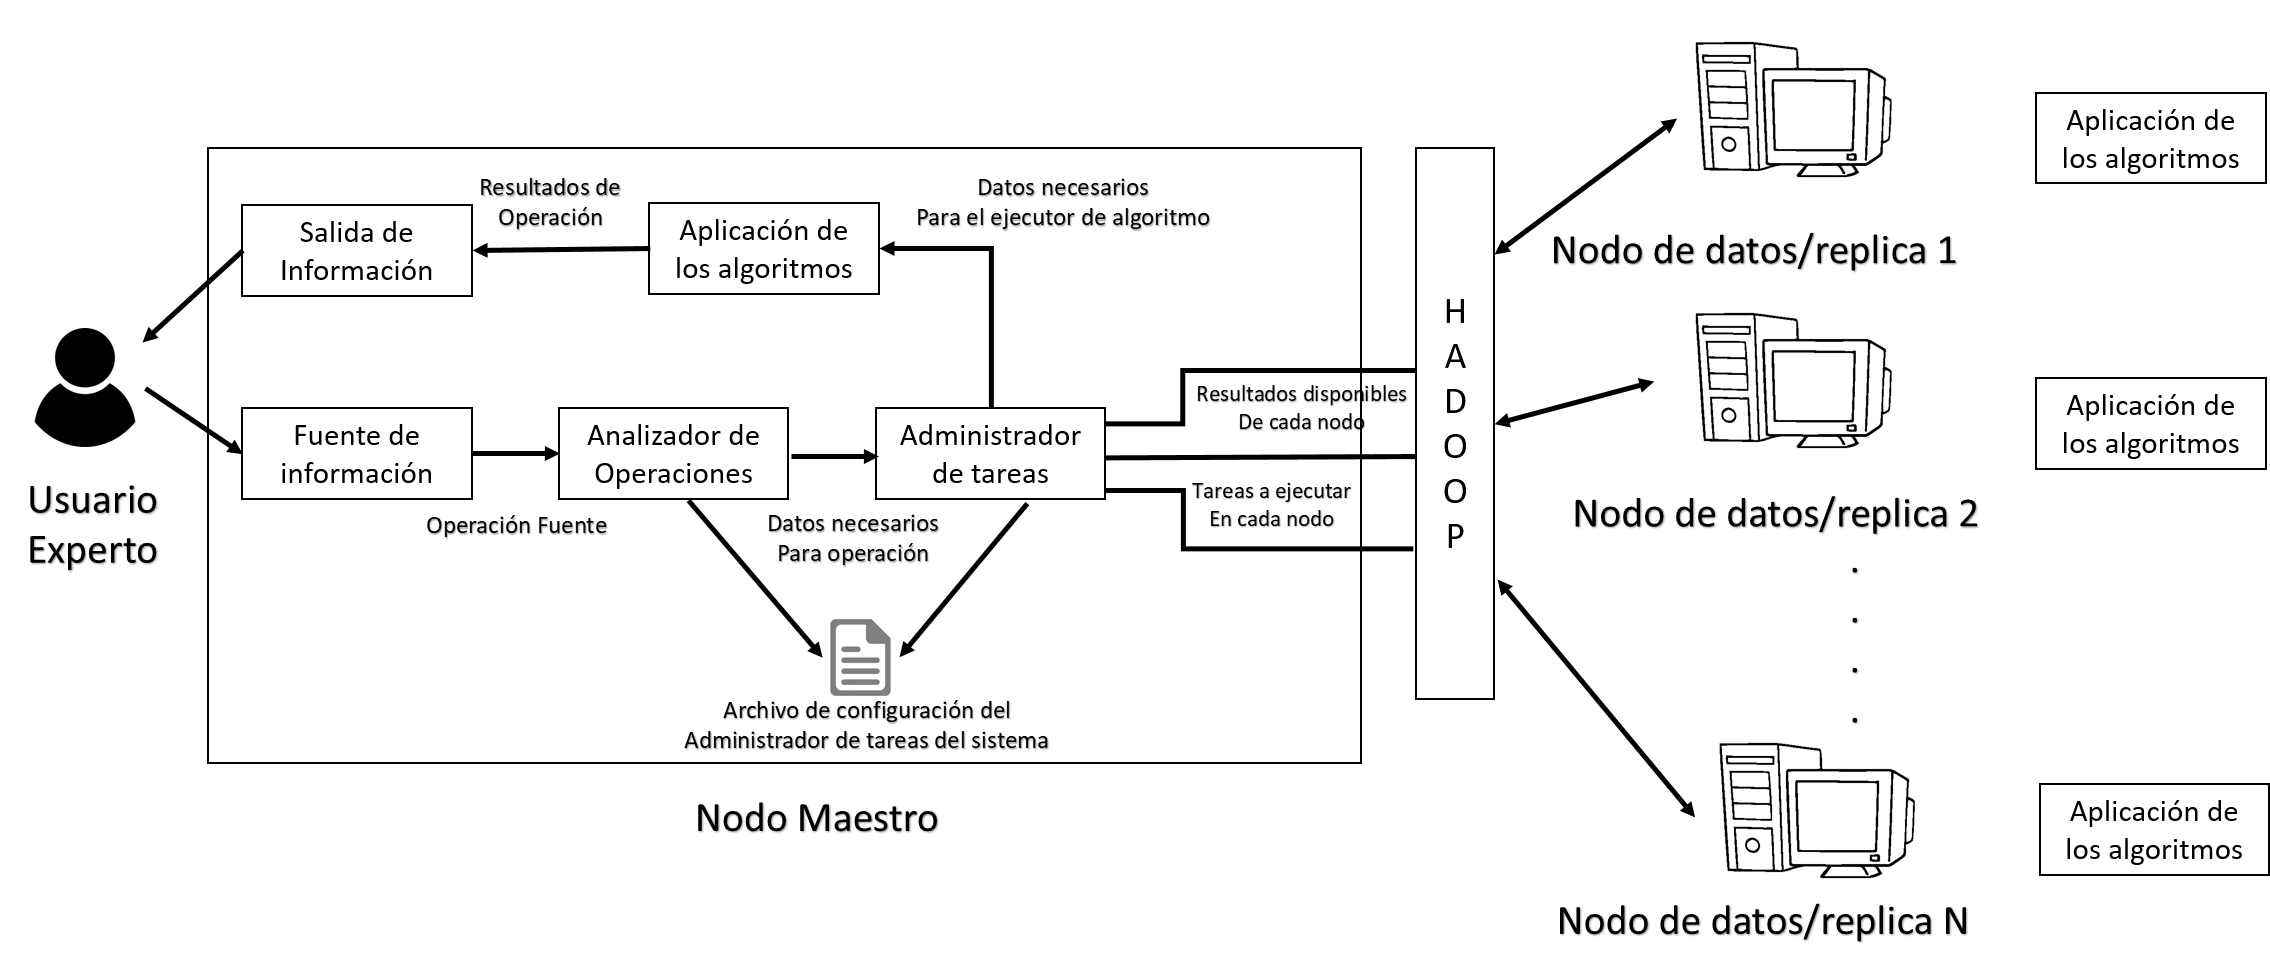
\includegraphics[height=0.3\textheight]{capitulo1/images/im1.png}
		\caption{Arquitectura de la red distribuida}
		\label{fig:cap1}
	\end{center}
\end{figure}
\\ 
Con esta arquitectura será posible adaptar el ambiente de Big Data a diversos casos de estudio de las empresas, modificando únicamente archivos que serán destinados para la configuración de dichos
casos de estudio. 
\\
Esto sin tener que modificar la arquitectura del sistema ni entender su funcionamiento interno. Será posible
mantener muy bien separados los bloques de código que realizan cada actividad en el sistema para que en caso de algún fallo sea
más fácil detectar en dónde está ocurriendo.
\\
A continuación se explicarán cada uno de los bloques que conforman la arquitectura del sistema.
\begin{itemize}
	\item \textbf{Salida de información}: Es el bloque que se encarga de presentar el resultado final al usuario experto, luego de aplicar los algoritmos de Big Data sobre ellos.
	\item \textbf{Aplicación de los algoritmos}: Es el modulo que permite aplicar los algoritmos de minería de datos sobre los nodos de datos/replica a los datos. ademas de aplicar la función reduce con los resultados en el nodo maestro.
	El funcionamiento de la función reduce se explica en la sección del documento \ref{funcionreduce} dentro del capitulo \nameref{cap:Cap4}.
	\item \textbf{Fuente de información}: Es el modulo que recibe como dato de entrada el algoritmo de minería de datos a ejecutar del usuario conocida como operación fuente.
	\item \textbf{Analizador de operaciones}: Es el modulo encargado de revisar el caso de estudio en cuestión del usuario final para visualizar si es que se tienen que realizar ajustes en el \textbf{Archivo de configuración del recolector del sistema} además de revisar que todo se encuentre funcionando de manera adecuada y que sea posible ejecutar el algoritmo de minería de datos en este momento.
	Por otro lado también será el encargado de determinar la recomendación del algoritmo de minería de datos mas apropiado para cada caso de estudio.
	\item \textbf{Administrador de tareas}: es el encargado de administrar las tareas que llevará a cabo cada nodo de datos/replica así como también de recibir los resultados de las tareas que estos ejecuten de manera local en el nodo maestro.
	\item \textbf{Archivo de configuración del recolector del administrador de tareas }: Este archivo servirá para llevar a cabo el ajuste de los algoritmos de minería de datos a cada caso de estudio que quiera aplicar el usuario experto. sera necesario realizar algunos ajustes en el mismo para que los algoritmos puedan ser ejecutados de manera satisfactoria.
\end{itemize}
La arquitectura que se presenta por lo tanto, es una arquitectura del tipo maestro-esclavo, la cual es utilizada para el diseño de un cluster de Hadoop como se detalla en la sección \nameref{sect:hadoop} del marco teórico. 